\chapter{Temperatura e dilatazione termica}

Con questo capitolo cambiamo argomento: lasciamo la meccanica e cominciamo a studiare i fenomeni legati al \textbf{caldo} e al \textbf{freddo}. La parte della fisica che se ne occupa si chiama \textbf{termologia}.

Il primo passo è dare una definizione precisa di \textbf{temperatura} e imparare a misurarla; poi studiamo un effetto che quasi tutti i corpi mostrano quando la temperatura cambia: la \textbf{dilatazione termica}. Il \emph{calore} -- che cos'è, come si trasferisce, come si misura -- sarà l'argomento del capitolo successivo.

\section[La temperatura]{La temperatura}

\subsection{Agitazione termica}
La materia è fatta di \textbf{particelle} (atomi o molecole) che, qualunque sia lo stato di aggregazione, sono in continuo movimento: vibrano attorno a una posizione, oppure si spostano e si urtano fra loro. Questo movimento disordinato si chiama \textbf{agitazione termica}.

\begin{definizione}
La \textbf{temperatura} è un indice dello stato di agitazione termica di una sostanza: dice quanto velocemente, in media, si muovono le sue particelle. Più grande è l'agitazione termica, maggiore è la temperatura.
\end{definizione}

Gli atomi di un cucchiaio caldo vibrano più velocemente di quelli dello stesso cucchiaio da freddo; le molecole dell'aria di una stanza calda si muovono più in fretta di quelle di una stanza fredda.

\subsection{L'equilibrio termico}
Quando un corpo caldo viene messo a contatto con un corpo freddo, dopo un certo tempo i due corpi assumono la \textbf{stessa temperatura}: si dice che hanno raggiunto l'\textbf{equilibrio termico}.

Le sensazioni di caldo e freddo che ci trasmette la pelle sono soggettive e poco affidabili: la stessa acqua tiepida sembra calda alla mano che era al freddo e fredda alla mano che era al caldo. Per avere un'informazione oggettiva bisogna \emph{misurare} la temperatura con un \textbf{termometro}.

\subsection{Le scale termometriche}
Un termometro si costruisce fissando due \textbf{temperature di riferimento} facilmente riproducibili, assegnando loro due numeri e dividendo l'intervallo in parti uguali.

\begin{definizione}
Nella \textbf{scala Celsius} (o centigrada) si assegna il valore $0$ alla temperatura del \emph{ghiaccio fondente} e il valore $100$ a quella dell'\emph{acqua bollente} (a pressione atmosferica). L'intervallo è diviso in $100$ parti, ognuna delle quali è un \textbf{grado Celsius} (simbolo \si{\celsius}).
\end{definizione}

\begin{definizione}
Nella \textbf{scala Kelvin} (la scala del Sistema Internazionale) l'unità -- il \textbf{kelvin} (simbolo \si{\kelvin}) -- ha la stessa ampiezza del grado Celsius, ma lo zero è spostato: al ghiaccio fondente si assegna $273{,}15$, all'acqua bollente $373{,}15$. Lo zero della scala Kelvin, $\SI{0}{\kelvin} = \SI{-273,15}{\celsius}$, si chiama \textbf{zero assoluto}: è la temperatura a cui l'agitazione termica si annullerebbe, e non può essere superata verso il basso.
\end{definizione}

Per passare da una temperatura espressa in gradi Celsius ($T_C$) alla stessa temperatura in kelvin ($T_K$), e viceversa:
\[ \colorboxed{ocre}{ T_K = T_C + 273{,}15, \qquad T_C = T_K - 273{,}15. } \]

\begin{figure}[!htbp]
    \centering
    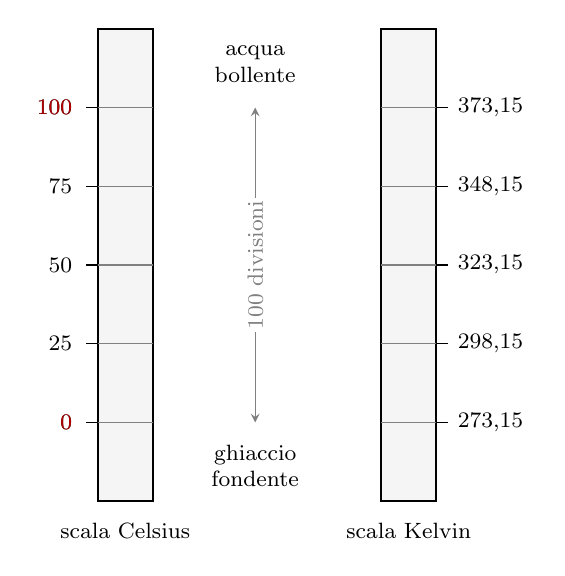
\begin{tikzpicture}[>=stealth]
        % due colonne verticali
        \foreach \x/\lab in {0/{scala Celsius}, 3.6/{scala Kelvin}}{
            \draw[thick,fill=gray!8] (\x,0) rectangle (\x+0.7,6);
            \node[below] at (\x+0.35,-0.15) {\footnotesize \lab};
        }
        % tacche Celsius: 0 (ghiaccio) a y=1, 100 (acqua) a y=5
        \foreach \y/\v in {1/0, 2/25, 3/50, 4/75, 5/100}{
            \draw (0,\y) -- (-0.15,\y) node[left]{\footnotesize \v\,\si{\celsius}};
            \draw[gray] (0,\y) -- (0.7,\y);
        }
        \node[left,red!70!black] at (-0.15,1) {\footnotesize $0\,\si{\celsius}$};
        \node[left,red!70!black] at (-0.15,5) {\footnotesize $100\,\si{\celsius}$};
        % tacche Kelvin
        \foreach \y/\v in {1/273{,}15, 2/298{,}15, 3/323{,}15, 4/348{,}15, 5/373{,}15}{
            \draw (4.3,\y) -- (4.45,\y) node[right]{\footnotesize \v\,\si{\kelvin}};
            \draw[gray] (3.6,\y) -- (4.3,\y);
        }
        % riferimenti
        \draw[<->,gray] (2.0,1) -- (2.0,5) node[midway,fill=white,inner sep=1pt,rotate=90]{\footnotesize $100$ divisioni};
        \node[align=center,font=\footnotesize] at (2.0,0.45) {ghiaccio\\fondente};
        \node[align=center,font=\footnotesize] at (2.0,5.55) {acqua\\bollente};
    \end{tikzpicture}
    \caption{Le scale Celsius e Kelvin: le divisioni hanno la stessa ampiezza, cambia solo la posizione dello zero. Una differenza di temperatura vale lo stesso numero nelle due scale.}
    \label{fig:scale-termometriche}
\end{figure}

\begin{remark}
Le due scale differiscono solo per la posizione dello zero, non per l'ampiezza delle divisioni. Perciò una \emph{differenza} di temperatura vale lo stesso numero nelle due scale:
\[ \Delta T_K = \Delta T_C. \]
Un aumento di \SI{10}{\celsius} è anche un aumento di \SI{10}{\kelvin}. Questo sarà comodo nelle formule della dilatazione e della termologia, dove compaiono sempre \emph{variazioni} di temperatura.
\end{remark}

\subsection{La scala Fahrenheit}
Nei paesi anglosassoni si usa la \textbf{scala Fahrenheit} (\si{\fahrenheit}): il ghiaccio fondente è a \SI{32}{\fahrenheit} e l'acqua bollente a \SI{212}{\fahrenheit}. La conversione con i gradi Celsius è
\[ T_F = \frac{9}{5}\,T_C + 32, \qquad T_C = \frac{5}{9}\,(T_F - 32). \]

\begin{testexample}[\thetcbcounter \, Qualche conversione]
La temperatura di un'aula è \SI{20}{\celsius}. In kelvin:
\[ T_K = 20 + 273{,}15 = \SI{293,15}{\kelvin}. \]
La temperatura del corpo umano è \SI{37}{\celsius}. In gradi Fahrenheit:
\[ T_F = \frac{9}{5}\cdot 37 + 32 = 66{,}6 + 32 = \SI{98,6}{\fahrenheit}. \]
Una previsione di \SI{55}{\fahrenheit} negli Stati Uniti corrisponde a
\[ T_C = \frac{5}{9}\,(55 - 32) = \frac{5}{9}\cdot 23 \approx \SI{13}{\celsius}: \]
una giornata fresca, non torrida.
\end{testexample}

\begin{esercizio}
Converti in kelvin le temperature \SI{0}{\celsius}, \SI{25}{\celsius}, \SI{-18}{\celsius} e \SI{100}{\celsius}.\\
\risp{$273{,}15$; \; $298{,}15$; \; $255{,}15$; \; $373{,}15$ (K)}
\end{esercizio}

\begin{esercizio}
Converti in gradi Celsius le temperature \SI{300}{\kelvin}, \SI{195}{\kelvin} (sublimazione della CO$_2$) e \SI{0}{\kelvin}.\\
\risp{$26{,}85\,\si{\celsius}$; \; $-78{,}15\,\si{\celsius}$; \; $-273{,}15\,\si{\celsius}$}
\end{esercizio}

\begin{esercizio}
In una giornata estiva la massima a Roma è \SI{37}{\celsius}, a Londra è \SI{295}{\kelvin}. In entrambe le città la minima è \SI{9}{\celsius} più bassa della massima. Calcola le due minime in gradi Celsius e l'escursione termica in kelvin.\\
\risp{Roma: min $\SI{28}{\celsius}$; \; Londra: max $\SI{21,85}{\celsius}$, min $\approx \SI{12,85}{\celsius}$; \; escursione $\Delta T = \SI{9}{\kelvin}$ in entrambe}
\end{esercizio}

\begin{esercizio}
Un termometro segna \SI{25}{\celsius}. Esprimi questa temperatura in gradi Fahrenheit. A quale temperatura le scale Celsius e Fahrenheit segnano lo stesso numero?\\
\risp{$T_F = \tfrac95\cdot 25 + 32 = \SI{77}{\fahrenheit}$; \; uguali quando $T = \tfrac95 T + 32 \Rightarrow T = -40$ (cioè $\SI{-40}{\celsius} = \SI{-40}{\fahrenheit}$)}
\end{esercizio}

\begin{esercizio}
La temperatura media della superficie del Sole è circa \SI{5800}{\kelvin}. Quanto vale in gradi Celsius? Ha molta importanza, a queste temperature, la differenza fra le due scale?\\
\risp{$\approx \SI{5527}{\celsius}$; \; no, la differenza di $273$ è trascurabile rispetto al valore}
\end{esercizio}

\section[La dilatazione termica]{La dilatazione termica}

La colonnina di liquido di un termometro si allunga quando viene riscaldata. È un caso particolare di un fenomeno generale: quasi tutte le sostanze, riscaldandosi, aumentano le proprie dimensioni. Questo fenomeno si chiama \textbf{dilatazione termica}.

\subsection{La dilatazione lineare}
Se un corpo solido ha una dimensione molto più grande delle altre (un filo, una sbarra, un binario), la dilatazione si nota soprattutto lungo quella direzione: si parla allora di \textbf{dilatazione lineare}.

Prendiamo una sbarra di lunghezza iniziale $l_0$ alla temperatura $T_0$. La scaldiamo fino a una temperatura $T$: la lunghezza diventa $l$. L'allungamento è $\Delta l = l - l_0$ e la variazione di temperatura è $\Delta T = T - T_0$.

\begin{definizione}
\textbf{Legge della dilatazione lineare.} L'allungamento $\Delta l$ di un corpo riscaldato è:
\begin{itemize}
    \item direttamente proporzionale alla lunghezza iniziale $l_0$;
    \item direttamente proporzionale alla variazione di temperatura $\Delta T$;
    \item legato alla natura della sostanza attraverso un coefficiente $\lambda$ (``lambda''), detto \textbf{coefficiente di dilatazione lineare}:
\end{itemize}
\[ \colorboxed{ocre}{ \Delta l = \lambda\,l_0\,\Delta T. } \]
Il coefficiente $\lambda$ si misura in $\si{\kelvin}^{-1}$ (o, indifferentemente, in $\si{\celsius}^{-1}$, dato che $\Delta T$ vale lo stesso nelle due scale).
\end{definizione}

\begin{table}[!htbp]
    \centering
    \begin{tabular}{lc}
        \toprule
        sostanza & $\lambda$ $(\si{\celsius}^{-1})$ \\
        \midrule
        alluminio & $2{,}4 \times 10^{-5}$ \\
        argento & $1{,}9 \times 10^{-5}$ \\
        ferro / acciaio & $1{,}2 \times 10^{-5}$ \\
        rame & $1{,}7 \times 10^{-5}$ \\
        vetro comune & $0{,}9 \times 10^{-5}$ \\
        vetro pyrex & $0{,}3 \times 10^{-5}$ \\
        cemento & $1{,}0 \times 10^{-5}$ \\
        \bottomrule
    \end{tabular}
    \caption{Coefficiente di dilatazione lineare di alcuni solidi (valori indicativi a temperatura ambiente).}
    \label{tab:dilatazione-lineare}
\end{table}

\begin{figure}[!htbp]
    \centering
    \begin{tikzpicture}[>=stealth]
        % sbarra a T0
        \draw[fill=gray!25] (0,1.2) rectangle (5,1.6);
        \draw[<->] (0,2.0) -- (5,2.0) node[midway,above]{$l_0$};
        \node[left] at (-0.15,1.4) {$T_0$};
        % sbarra a T (piu lunga)
        \draw[fill=ocre!30] (0,0) rectangle (5.9,0.4);
        \draw[<->] (0,-0.4) -- (5.9,-0.4) node[midway,below]{$l$};
        \node[left] at (-0.15,0.2) {$T > T_0$};
        \draw[<->] (5,0.55) -- (5.9,0.55) node[midway,above,font=\footnotesize]{$\Delta l$};
        \draw[gray,dashed] (5,0) -- (5,1.2);
    \end{tikzpicture}
    \caption{Dilatazione lineare: scaldata di $\Delta T$, la sbarra si allunga di $\Delta l = \lambda\,l_0\,\Delta T$. Raffreddandola ($\Delta T < 0$) si accorcia.}
    \label{fig:dilatazione-lineare}
\end{figure}

\begin{remark}
Poiché $l_0$ e $\lambda$ sono positivi, il segno di $\Delta l$ è quello di $\Delta T$: un corpo riscaldato si allunga, un corpo raffreddato si accorcia. I coefficienti sono molto piccoli (dell'ordine di $10^{-5}$), quindi le variazioni di lunghezza sono piccole in termini relativi -- ma non trascurabili su grandi strutture: per questo i binari, i ponti e le tubature hanno i \textbf{giunti di dilatazione}, spazi vuoti che permettono al materiale di allungarsi senza deformarsi.
\end{remark}

\begin{testexample}[\thetcbcounter \, L'allungamento di un binario]
Un binario di acciaio ($\lambda = \num{1,2e-5}\,\si{\celsius}^{-1}$) è lungo \SI{25}{\metre} a \SI{10}{\celsius}. In una giornata d'estate la sua temperatura sale a \SI{45}{\celsius}. Di quanto si allunga?
\[ \Delta l = \lambda\,l_0\,\Delta T = \num{1,2e-5} \cdot 25 \cdot 35 \approx \SI{1,05e-2}{\metre} \approx \SI{1,1}{\centi\metre}. \]
Poco più di un centimetro: se i binari fossero saldati senza spazi, questa dilatazione li farebbe deformare.
\end{testexample}

\begin{testexample}[\thetcbcounter \, A quale temperatura?]
Un fabbro deve allungare di \SI{5,0}{\milli\metre} un tondino di acciaio lungo \SI{2,50}{\metre} a \SI{20}{\celsius}. A quale temperatura deve portarlo?

Ricaviamo $\Delta T$ dalla legge della dilatazione:
\[ \Delta T = \frac{\Delta l}{\lambda\,l_0} = \frac{\SI{5,0e-3}{\metre}}{\num{1,2e-5} \cdot \SI{2,50}{\metre}} \approx \SI{167}{\celsius}. \]
La temperatura finale è $T = 20 + 167 \approx \SI{187}{\celsius}$.
\end{testexample}

\subsection{La dilatazione volumica dei solidi}
Se il corpo non ha una dimensione dominante (un cubo, una sfera), la dilatazione si manifesta in tutte le direzioni e conviene ragionare sul \textbf{volume}.

\begin{definizione}
\textbf{Legge della dilatazione volumica.} La variazione di volume $\Delta V$ di un solido riscaldato è direttamente proporzionale al volume iniziale $V_0$, alla variazione di temperatura $\Delta T$ e a un coefficiente $k$ caratteristico della sostanza, detto \textbf{coefficiente di dilatazione volumica}:
\[ \colorboxed{ocre}{ \Delta V = k\,V_0\,\Delta T. } \]
Per un solido isotropo vale con buona approssimazione
\[ k \approx 3\,\lambda. \]
\end{definizione}

Il fattore $3$ si spiega notando che un cubo di lato $l_0$ ha volume $l_0^3$: se ogni lato aumenta di una piccola frazione, il volume aumenta di circa il \emph{triplo} di quella frazione.

\begin{remark}
La dilatazione riguarda anche i \textbf{fori} e le cavità: un anello metallico riscaldato non si ``stringe'', ma si allarga, esattamente come se il foro fosse fatto dello stesso materiale. Per questo un tappo di vetro incastrato in una bottiglia si libera scaldando il collo della bottiglia.
\end{remark}

\begin{testexample}[\thetcbcounter \, La sfera e l'anello]
Una sfera di alluminio ha diametro \SI{100,0}{\milli\metre} e passa (appena appena) attraverso un anello di diametro \SI{100,5}{\milli\metre}, entrambi a \SI{20}{\celsius}. A quale temperatura bisogna portare la sfera perché non passi più nell'anello?

Basta che il diametro della sfera arrivi a eguagliare quello dell'anello. Il diametro si dilata come una lunghezza:
\[ \Delta D = \lambda\,D_0\,\Delta T. \]
Vogliamo $\Delta D = 100{,}5 - 100{,}0 = \SI{0,5}{\milli\metre}$, quindi
\[ \Delta T = \frac{\Delta D}{\lambda\,D_0} = \frac{0{,}5}{\num{2,4e-5} \cdot 100{,}0} \approx \SI{208}{\celsius}. \]
La sfera va portata a $T \approx 20 + 208 \approx \SI{228}{\celsius}$.
\end{testexample}

\subsection{La dilatazione dei liquidi e l'anomalia dell'acqua}
Anche i liquidi si dilatano secondo la legge $\Delta V = k\,V_0\,\Delta T$, ma con coefficienti $k$ molto maggiori di quelli dei solidi (perché le forze fra le molecole sono più deboli). È il motivo per cui il liquido di un termometro sale visibilmente nel tubicino mentre il vetro attorno si dilata pochissimo.

\begin{table}[!htbp]
    \centering
    \begin{tabular}{lc}
        \toprule
        liquido & $k$ $(\si{\celsius}^{-1})$ \\
        \midrule
        mercurio & $1{,}8 \times 10^{-4}$ \\
        acqua (sopra i \SI{4}{\celsius}) & $2{,}1 \times 10^{-4}$ \\
        alcol etilico & $1{,}1 \times 10^{-3}$ \\
        glicerina & $5{,}0 \times 10^{-4}$ \\
        \bottomrule
    \end{tabular}
    \caption{Coefficiente di dilatazione volumica di alcuni liquidi.}
    \label{tab:dilatazione-liquidi}
\end{table}

L'\textbf{acqua} fa eccezione. Fra \SI{0}{\celsius} e \SI{4}{\celsius}, invece di dilatarsi scaldandosi, si \emph{contrae}: il suo volume è \textbf{minimo a \SI{4}{\celsius}} (figura~\ref{fig:anomalia-acqua}). Sopra i \SI{4}{\celsius} si comporta come gli altri liquidi. Questo \textbf{comportamento anomalo} ha conseguenze importanti: l'acqua più densa (a \SI{4}{\celsius}) va a fondo, mentre quella più fredda resta in superficie e ghiaccia per prima. Un lago gela dall'alto e sul fondo resta acqua liquida a \SI{4}{\celsius}, permettendo la sopravvivenza di pesci e piante.

\begin{figure}[!htbp]
    \centering
    \begin{tikzpicture}
    \begin{axis}[
        width=0.72\linewidth, height=5cm,
        xlabel={temperatura (\si{\celsius})}, ylabel={volume},
        xmin=0, xmax=12, ymin=0, ymax=2.4,
        xtick={0,2,4,6,8,10,12}, ytick=\empty,
        axis lines=left, tick label style={font=\footnotesize},
        label style={font=\footnotesize}, clip=false,
    ]
    \addplot[ocre,very thick,samples=100,domain=0:12] {0.03*(x-4)^2 + 0.25};
    \draw[gray,dashed] (axis cs:4,0) -- (axis cs:4,1.15);
    \fill[ocre] (axis cs:4,0.25) circle (1.6pt);
    \node[font=\footnotesize,anchor=south] at (axis cs:4,1.2) {volume minimo};
    \end{axis}
    \end{tikzpicture}
    \caption{Comportamento anomalo dell'acqua: fra \SI{0}{\celsius} e \SI{4}{\celsius} il volume \emph{diminuisce} all'aumentare della temperatura. Il volume è minimo (la densità massima) a \SI{4}{\celsius}.}
    \label{fig:anomalia-acqua}
\end{figure}

\begin{testexample}[\thetcbcounter \, Un termometro a mercurio]
Il bulbo di un termometro contiene \SI{0,20}{\milli\litre} di mercurio ($k = \num{1,8e-4}\,\si{\celsius}^{-1}$) e il tubicino ha sezione $A = \SI{0,040}{\milli\metre\squared}$. Di quanto sale la colonnina se la temperatura aumenta di \SI{8,0}{\celsius}? (Trascuriamo la dilatazione del vetro.)

Conviene lavorare in millimetri cubi: $\SI{0,20}{\milli\litre} = \SI{0,20}{\centi\metre\cubed} = \SI{200}{\milli\metre\cubed}$. La variazione di volume del mercurio è
\[ \Delta V = k\,V_0\,\Delta T = \num{1,8e-4} \cdot \SI{200}{\milli\metre\cubed} \cdot 8{,}0 \approx \SI{0,29}{\milli\metre\cubed}. \]
Questo volume in più si dispone nel tubicino formando una colonnina di altezza
\[ h = \frac{\Delta V}{A} = \frac{\SI{0,29}{\milli\metre\cubed}}{\SI{0,040}{\milli\metre\squared}} \approx \SI{7,2}{\milli\metre}. \]
Su un intervallo di soli \SI{8}{\celsius}, il mercurio percorre \SI{7}{\milli\metre} di scala: la dilatazione, minuscola in valore assoluto, è ben leggibile.
\end{testexample}

\begin{esercizio}
Un cavo di rame ($\lambda = \num{1,7e-5}\,\si{\celsius}^{-1}$) di una linea elettrica è lungo \SI{80}{\metre} a \SI{15}{\celsius}. Di quanto si allunga se d'estate arriva a \SI{40}{\celsius}?\\
\risp{$\Delta l = \num{1,7e-5} \cdot 80 \cdot 25 \approx \SI{3,4e-2}{\metre} = \SI{3,4}{\centi\metre}$}
\end{esercizio}

\begin{esercizio}
Un'impalcatura di ferro ($\lambda = \num{1,2e-5}\,\si{\celsius}^{-1}$) è alta \SI{24,00}{\metre} a \SI{20}{\celsius}. In estate può arrivare a \SI{50}{\celsius}. Qual è la massima altezza che può raggiungere?\\
\risp{$\Delta l = \num{1,2e-5} \cdot 24{,}00 \cdot 30 \approx \SI{8,6e-3}{\metre}$; \; altezza $\approx \SI{24,01}{\metre}$}
\end{esercizio}

\begin{esercizio}
Un cubo di alluminio ha lato \SI{1,000}{\metre} a \SI{100}{\celsius} e viene portato a \SI{300}{\celsius}. Qual è la lunghezza finale dei suoi spigoli?\\
\risp{$\Delta l = \num{2,4e-5} \cdot 1{,}000 \cdot 200 = \SI{4,8e-3}{\metre}$; \; lato $\approx \SI{1,005}{\metre}$}
\end{esercizio}

\begin{esercizio}
Una sfera di ottone ($k = \num{6,0e-5}\,\si{\celsius}^{-1}$) ha volume \SI{800}{\centi\metre\cubed} a \SI{20}{\celsius}. Qual è il suo volume a \SI{120}{\celsius}?\\
\risp{$\Delta V = \num{6,0e-5} \cdot 800 \cdot 100 = \SI{4,8}{\centi\metre\cubed}$; \; $V \approx \SI{804,8}{\centi\metre\cubed}$}
\end{esercizio}

\begin{esercizio}
Un ponte di cemento ($\lambda = \num{1,0e-5}\,\si{\celsius}^{-1}$) lungo \SI{120}{\metre} è progettato per lavorare fra \SI{-10}{\celsius} e \SI{40}{\celsius}. Quanto deve essere largo, come minimo, il giunto di dilatazione?\\
\risp{$\Delta l = \num{1,0e-5} \cdot 120 \cdot 50 = \SI{6,0e-2}{\metre} = \SI{6,0}{\centi\metre}$}
\end{esercizio}

\begin{esercizio}
Un recipiente di vetro pyrex ($\lambda = \num{0,3e-5}\,\si{\celsius}^{-1}$) è pieno raso di \SI{500}{\centi\metre\cubed} di alcol etilico ($k = \num{1,1e-3}\,\si{\celsius}^{-1}$) a \SI{20}{\celsius}. Scaldando il tutto di \SI{15}{\celsius}, quanto alcol trabocca? (Confronta la dilatazione dell'alcol con quella della cavità di vetro, $k_{\text{vetro}} \approx 3\lambda$.)\\
\risp{$\Delta V_{\text{alcol}} = \num{1,1e-3}\cdot 500 \cdot 15 \approx \SI{8,3}{\centi\metre\cubed}$; \; $\Delta V_{\text{cavità}} = \num{0,9e-5}\cdot 500 \cdot 15 \approx \SI{0,07}{\centi\metre\cubed}$; \; trabocca $\approx \SI{8,2}{\centi\metre\cubed}$}
\end{esercizio}

\section{Problemi di riepilogo}

\begin{esercizio}
Converti \SI{68}{\fahrenheit} in gradi Celsius e in kelvin.\\
\risp{$T_C = \tfrac59(68 - 32) = \SI{20}{\celsius}$; \; $T_K = \SI{293,15}{\kelvin}$}
\end{esercizio}

\begin{esercizio}
La temperatura di un forno passa da \SI{20}{\celsius} a \SI{220}{\celsius}. Esprimi la temperatura iniziale, quella finale e la variazione in kelvin.\\
\risp{$293{,}15\,\si{\kelvin}$; \; $493{,}15\,\si{\kelvin}$; \; $\Delta T = \SI{200}{\kelvin}$}
\end{esercizio}

\begin{esercizio}
Un termometro difettoso segna \SI{2}{\celsius} nel ghiaccio fondente e \SI{102}{\celsius} nell'acqua bollente. Che temperatura reale corrisponde a una lettura di \SI{52}{\celsius}?\\
\risp{la scala è traslata di \SI{2}{\celsius} e ha la stessa ampiezza: temperatura reale $= 52 - 2 = \SI{50}{\celsius}$}
\end{esercizio}

\begin{esercizio}
Un binario di acciaio lungo \SI{30}{\metre} viene posato a \SI{8}{\celsius}. Quale spazio va lasciato all'estremità perché il binario possa dilatarsi fino a \SI{43}{\celsius} senza deformarsi? ($\lambda = \num{1,2e-5}\,\si{\celsius}^{-1}$)\\
\risp{$\Delta l = \num{1,2e-5} \cdot 30 \cdot 35 \approx \SI{1,3e-2}{\metre} \approx \SI{1,3}{\centi\metre}$}
\end{esercizio}

\begin{esercizio}
Un filo di ferro lungo \SI{2,0}{\metre} a \SI{20}{\celsius} viene raffreddato fino a \SI{-30}{\celsius}. Di quanto si accorcia? ($\lambda = \num{1,2e-5}\,\si{\celsius}^{-1}$)\\
\risp{$\Delta l = \num{1,2e-5} \cdot 2{,}0 \cdot (-50) = \SI{-1,2e-3}{\metre} = \SI{-1,2}{\milli\metre}$ (si accorcia di \SI{1,2}{\milli\metre})}
\end{esercizio}

\begin{esercizio}
Una lastra quadrata di alluminio ha lato \SI{50,0}{\centi\metre} a \SI{25}{\celsius}. Qual è la sua area a \SI{125}{\celsius}? (La dilatazione superficiale ha coefficiente $\approx 2\lambda$.) ($\lambda = \num{2,4e-5}\,\si{\celsius}^{-1}$)\\
\risp{$\Delta A = 2\lambda\,A_0\,\Delta T = \num{4,8e-5} \cdot 2500 \cdot 100 = \SI{12}{\centi\metre\squared}$; \; $A \approx \SI{2512}{\centi\metre\squared}$}
\end{esercizio}

\begin{esercizio}
Un pendolo di un orologio è un'asta di acciaio; a \SI{20}{\celsius} ha lunghezza \SI{0,994}{\metre} e periodo esatto. D'estate la temperatura sale a \SI{35}{\celsius}. Di quanto si allunga l'asta? L'orologio anticipa o ritarda? ($\lambda = \num{1,2e-5}\,\si{\celsius}^{-1}$)\\
\risp{$\Delta l = \num{1,2e-5} \cdot 0{,}994 \cdot 15 \approx \SI{1,8e-4}{\metre}$; \; l'asta si allunga, $T = 2\pi\sqrt{l/g}$ cresce, l'orologio \textbf{ritarda}}
\end{esercizio}

\begin{esercizio}
Un serbatoio di acciaio contiene \SI{60}{\litre} di benzina ($k = \num{9,5e-4}\,\si{\celsius}^{-1}$) a \SI{10}{\celsius}. Il serbatoio viene riempito raso. Se la temperatura sale a \SI{35}{\celsius}, quanta benzina trabocca? (Trascura la dilatazione del serbatoio.)\\
\risp{$\Delta V = \num{9,5e-4} \cdot 60 \cdot 25 \approx \SI{1,4}{\litre}$}
\end{esercizio}

\begin{esercizio}
Due sbarre, una di alluminio e una di ferro, hanno la stessa lunghezza \SI{1,00}{\metre} a \SI{0}{\celsius}. A quale temperatura la sbarra di alluminio è \SI{1,0}{\milli\metre} più lunga di quella di ferro? ($\lambda_{\text{Al}} = \SI{2,4e-5}{}$, $\lambda_{\text{Fe}} = \SI{1,2e-5}{}$, in $\si{\celsius}^{-1}$)\\
\risp{$(\lambda_{\text{Al}} - \lambda_{\text{Fe}})\,l_0\,\Delta T = \SI{1,0e-3}{\metre} \Rightarrow \Delta T = \dfrac{\num{1,0e-3}}{\num{1,2e-5} \cdot 1{,}00} \approx \SI{83}{\celsius}$}
\end{esercizio}

\begin{esercizio}
Il diametro di un foro in una piastra di rame è \SI{20,00}{\milli\metre} a \SI{20}{\celsius}. Quanto vale a \SI{220}{\celsius}? ($\lambda = \num{1,7e-5}\,\si{\celsius}^{-1}$)\\
\risp{$\Delta D = \num{1,7e-5} \cdot 20{,}00 \cdot 200 \approx \SI{0,068}{\milli\metre}$; \; $D \approx \SI{20,07}{\milli\metre}$ (il foro si allarga)}
\end{esercizio}

\begin{esercizio}
Perché è pericoloso versare acqua bollente in un bicchiere di vetro comune, ma non in uno di pyrex?\\
\risp{il vetro comune ha $\lambda$ tre volte quello del pyrex: la parte interna, scaldandosi bruscamente, si dilata molto più di quella esterna e il vetro si può rompere. Il pyrex si dilata poco e sopporta lo shock termico}
\end{esercizio}

\begin{esercizio}
Un cilindro di acciaio ha diametro \SI{50,00}{\milli\metre} e deve essere inserito in un foro di diametro \SI{49,98}{\milli\metre} in una piastra di acciaio, entrambi a \SI{20}{\celsius}. Conviene scaldare la piastra o raffreddare il cilindro? Di quanti gradi, in ciascun caso? ($\lambda = \num{1,2e-5}\,\si{\celsius}^{-1}$)\\
\risp{scaldare la piastra: $\Delta T = \dfrac{0{,}02}{\num{1,2e-5}\cdot 49{,}98} \approx \SI{33}{\celsius}$ (a \SI{53}{\celsius}); \; oppure raffreddare il cilindro dello stesso $\Delta T$ (a $\approx \SI{-13}{\celsius}$)}
\end{esercizio}

\begin{esercizio}
Una lamina bimetallica è formata da una striscia di ferro e una di ottone ($\lambda_{\text{ottone}} = \SI{1,9e-5}{}$, $\lambda_{\text{Fe}} = \SI{1,2e-5}{}$, in $\si{\celsius}^{-1}$) saldate insieme. Che cosa succede quando la lamina viene scaldata? A che cosa può servire?\\
\risp{l'ottone si allunga di più, quindi la lamina si incurva (verso il lato del ferro); serve da interruttore automatico nei termostati (apre/chiude un contatto in base alla temperatura)}
\end{esercizio}

\begin{esercizio}
La densità del ferro a \SI{20}{\celsius} è \SI{7,87}{\gram\per\centi\metre\cubed}. Qual è, approssimativamente, la sua densità a \SI{520}{\celsius}? (La massa non cambia, il volume aumenta di $\Delta V = 3\lambda\,V_0\,\Delta T$.) ($\lambda = \num{1,2e-5}\,\si{\celsius}^{-1}$)\\
\risp{$\Delta V/V_0 = 3 \cdot \num{1,2e-5} \cdot 500 = 0{,}018$; \; $\rho \approx \dfrac{7{,}87}{1{,}018} \approx \SI{7,73}{\gram\per\centi\metre\cubed}$}
\end{esercizio}

\begin{esercizio}
Un tubo dell'acqua in rame è lungo \SI{12}{\metre} quando l'acqua che lo attraversa è a \SI{55}{\celsius}. Di quanto era più corto quando, prima dell'uso, era a \SI{15}{\celsius}? ($\lambda = \num{1,7e-5}\,\si{\celsius}^{-1}$)\\
\risp{$\Delta l = \num{1,7e-5} \cdot 12 \cdot 40 \approx \SI{8,2e-3}{\metre} \approx \SI{8}{\milli\metre}$}
\end{esercizio}

\begin{esercizio}
Un recipiente di alluminio ha capacità \SI{2,000}{\litre} a \SI{20}{\celsius}. Vi si versano \SI{2,000}{\litre} di acqua a \SI{20}{\celsius}. Scaldando il tutto a \SI{80}{\celsius}, l'acqua trabocca? Di quanto? ($k_{\text{acqua}} = \SI{2,1e-4}{}$, $\lambda_{\text{Al}} = \SI{2,4e-5}{}$, in $\si{\celsius}^{-1}$)\\
\risp{$\Delta V_{\text{acqua}} = \num{2,1e-4} \cdot 2{,}000 \cdot 60 \approx \SI{25}{\milli\litre}$; \; $\Delta V_{\text{recipiente}} = 3\lambda\,V_0\,\Delta T = \num{7,2e-5} \cdot 2{,}000 \cdot 60 \approx \SI{8,6}{\milli\litre}$; \; trabocca $\approx \SI{17}{\milli\litre}$}
\end{esercizio}

\begin{esercizio}
Spiega, in termini di agitazione termica, perché scaldando un gas in un recipiente chiuso e rigido la sua pressione aumenta.\\
\risp{scaldando, le molecole si muovono più velocemente e urtano le pareti più spesso e con più forza; la pressione, che è la forza per unità di superficie dovuta a questi urti, aumenta}
\end{esercizio}

\begin{esercizio}
Un anello di acciaio ha diametro interno \SI{60,00}{\milli\metre} a \SI{20}{\celsius} e va calettato (montato a caldo) su un albero di diametro \SI{60,05}{\milli\metre}. A quale temperatura va portato l'anello perché scivoli sull'albero? ($\lambda = \num{1,2e-5}\,\si{\celsius}^{-1}$)\\
\risp{$\Delta T = \dfrac{0{,}05}{\num{1,2e-5} \cdot 60{,}00} \approx \SI{69}{\celsius}$; \; $T \approx \SI{89}{\celsius}$}
\end{esercizio}

\begin{esercizio}
A quale temperatura in kelvin l'agitazione termica di una sostanza si annullerebbe del tutto? Perché nella pratica non si può raggiungere?\\
\risp{a \SI{0}{\kelvin} (zero assoluto, $\SI{-273,15}{\celsius}$); \; è un limite che si può solo avvicinare: raffreddare significa sottrarre agitazione termica, e avvicinandosi allo zero diventa sempre più difficile toglierne ancora}
\end{esercizio}

\begin{esercizio}
Una barra di ottone lunga \SI{1,50}{\metre} a \SI{25}{\celsius} si allunga di \SI{0,90}{\milli\metre} quando viene scaldata. Di quanti gradi è aumentata la temperatura? ($\lambda_{\text{ottone}} = \num{2,0e-5}\,\si{\celsius}^{-1}$)\\
\risp{$\Delta T = \dfrac{\num{0,90e-3}}{\num{2,0e-5} \cdot 1{,}50} = \SI{30}{\celsius}$; \; $T = \SI{55}{\celsius}$}
\end{esercizio}
